\documentclass[twocolumn]{revtex4}

\usepackage[]{graphicx}

\begin{document}

\title{Can you get away from the Velociraptor with a head start?}

\author{Santana Vicencio-LaBarre}
\affiliation{Siena College, Loudonville, NY}
\date{\today}

\begin{abstract}
This project was meant to find the likely-hood that a simple human, we'll call him Jimmy, would be able to escape a vicious velociraptor. The velociraptor was traveling at a velocity of 18 m/s while Jimmy was only traveling at 3 m/s luckily the Jimmy was given a 30 meter head start. But the second question asks you to find out when the raptor is able to catch up to you. The third question gets a little more difficult when you find that the raptor will only start to bite Jimmy when he his 1 meter away, you then must figure out how long in seconds and how far in meters Jimmy was able to travel before the raptor is close enough to bite. In the fourth question you must figure out the probability that Jimmy will get bitten by the raptor, luckily each time the raptor misses he looses a bit of his accuracy since he's getting more and more frustrated. 


\end{abstract}


\maketitle

\section{Introduction}

In this write up I will explain the point of the analysis, explain the algorithms, write out the equations and derivations I used, and include all the plots I made in python. 


\section{Question 1:Position vs. Time} 
In the first question I had to import matplotlib.pylab as plt in order to make the plot. I also needed to import numpy as np in order to make my array(list) for the time Jimmy and raptor were running. 

\subsection{Equations used to find position}

In order to find the position of the human and raptor I used the equation \textbf{position = v*time} for Jimmy's position I added 30 to the equation since there was a 30 meter head start.$$x_f = x_i \times t + 30 $$ 

\subsection{Plotting}
When plotting this Position Vs. Time graph I was sure label both the x and y axis as well as include a title "Human vs Raptor Position \& time". I also included a legend in order to specify which line went with either Jimmy or the raptor.


\subsection{Human Vs. Raptor Position \& Time plot}
%\graphicspath { {Desktop/github_repos/final_project/Final/} }
\begin{figure}
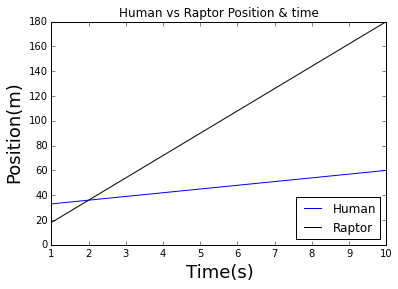
\includegraphics[width=0.5\textwidth]{Jimmy_Graph.png}
\caption {This is the plot from question one which shows the 	position and time of Jimmy and the Raptor. Jimmy is the blue line and the raptor is the black.}
\label{fig:Position vs. Time}
\end{figure}


\section{Question 2: When will you be caught?}

In this question I used a function to find how many meters Jimmy could travel before the raptor got him, as well as figuring out the time in seconds it took for the raptor to catch up. 

\subsection{Function explanation}

I called my function for this section, "gotcha" and i stated that for i in t if Jimmy and the raptors position equal each other return the time and position at which they do. I ended up getting the output that Jimmy ran 36 meters before the raptor caught him and the time that passed was 2 seconds. 

\section{Question 3: When will the raptor strike}

In this question I took a similar approach as question 2 but instead of having the positions equal each other I set the function to return the time and distance when the raptor positions minus Jimmy's position was less than or equal to 1. Then i added an arrow to my plot from question 1 to indicate where the raptor would be 1 meter behind Jimmy.As a result I got that Jimmy ran 33.0 meters in 1.0 seconds before the raptor was 1 meter behind him.

\section{Question 4: Will the raptor bite Jimmy?}

For question 4 I used a function with if and elif statements, and the np.random.randint code to get 100 random integers to find the probability Jimmy would be bit. 

\subsection{The code}

I set up a function in this question called "free" I made three different bites and had 100 random integers assigned to each. i then used 1 if statement paired with 2 elif statements and an else statement to assign the percent chance Jimmy would be bit. I set the first bite <=20 return "raptor food" and so on for the second and third bite but for the second bite it was <= 15, and for the this is was <=7. For my else statement i returned "you're safe!!!" because if Jimmy avoided the raptor after all three bites he would get away. 

\subsection{Probability}

Now to find the probability i used a for loop. I set raptor-food and safe equal to 0. Then i to i+=1 and t to t=free() which allowed for me to use and if and elif statement to find the probability. if t == "raptor food" then raptor food +=1 elif t == "you're safe!!!' safe +=1. By calling my function from above i used "freechance = (safe/float(1000))*100 to find the final probability which changes a little each time, but it roughly 61.20 percent 

\subsection{Plot With arrow}
\begin{figure}
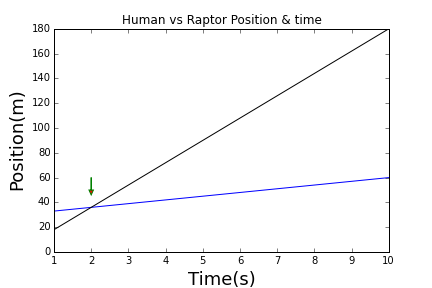
\includegraphics[width=0.5\textwidth]{Jimmy_Graph_Arrow.png}
\caption{This is the plot from question three which is the same as the plot from question one but includes an arrow to identify where the raptor is 1 meter behind Jimmy.}
\label{fig:Position vs. Time with arrow}
\end{figure}

\section{Conclusion}
This final project was most certainly a pain in the butt. It gave me a great feeling of accomplishment when i was able to fix the error in my code, or get my function to return the correct number. This project made me realize how much information I actually learned this semester, and some fun ways to use it. Now the big question of this project was if you (Jimmy) would be able to escape a velociraptor if you had a head start. Luckily the out come of this project shows that if Jimmy has a head start he's most likely going to get away from this raptor. 



\end{document}
